% !TeX spellcheck = pt_BR
% Observação lista de abreviaturas e símbolos:
% faz-se necessário executar os seguintes comandos no terminal (na pasta
% ue estão os arquivos) 
% makeindex -s pei.ist -o Dissertacao.lab Dissertacao.abx
% makeindex -s pei.ist -o Dissertacao.los Dissertacao.syx

\documentclass[msc]{pei}
\usepackage{array}
\usepackage{cmap}
\usepackage[utf8]{inputenc}
\usepackage[T1]{fontenc}
\usepackage{amsmath, amsfonts, amssymb, amstext, amsthm, mathtools, xfrac}
\usepackage[alf,abnt-etal-list=0]{abntex2cite}
\usepackage[brazil,nohints]{minitoc}
\usepackage{listings}
\usepackage{capitulos}
\usepackage{color}
\usepackage[font=footnotesize]{caption}
\usepackage{csquotes}
\usepackage{subcaption}
\usepackage{tabulary, array}
\usepackage{movie15}
\usepackage{rotating}
\usepackage{graphicx}
\usepackage{icomma}
\usepackage{epigraph}
\usepackage{pdfpages}
\usepackage[section]{placeins}
\usepackage{hyperref}
\usepackage{trivfloat}
\usepackage{tikz}
\usepackage{multirow}
\usepackage{placeins}
\usepackage{placeins}
\usepackage{makecell}
\usepackage{threeparttable}

\graphicspath{{imagens/}}
\newcommand{\figref}[1]{Figura~\ref{#1}}
\newcommand{\eqnref}[1]{Equa\c{c}\~{a}o~\eqref{#1}}
\newcommand{\tabref}[1]{Tabela~\ref{#1}}
\newcommand{\quadref}[1]{Quadro~\ref{#1}}
\newcommand{\exref}[1]{Ap\^{e}ndice~\ref{#1}}

%\newcommand\addtotoc[1]{\refstepcounter{dummy}\addcontentsline{toc}{chapter}{#1}}

\renewcommand{\lstlistingname}{Código}
\renewcommand{\lstlistlistingname}{Lista de Códigos}
\renewcommand\cellalign{cc}

\setcounter{MaxMatrixCols}{25}
\captionsetup{belowskip=6pt,aboveskip=4pt}
\setlength{\extrarowheight}{1.05pt}

%syntax highlighthing for EMSO codes
\lstdefinelanguage{EMSO}{
  morekeywords={
      Real,Boolean,Text,Integer,CalcObject,Model,FlowSheet,using, in, ext, out, as, to, end, switch, case, Switcher, time, diff, sin, cos, tan, exp, ln, log, if, else, asin, sqrt, outer, Plugin, Brief, Default, switchto, when, Optimization, Estimation, Reconciliation, CaseStudy, Sensitivity, Filter, GrossErrorTests, Significance, ObjectiveFunction, Global, Nodal, Measurements, RunTests, Statistics, BiLateral, Lower, Upper, Dynamic, false, true, TimeStart, TimeStep, TimeEnd, TimeUnit, final, Unit, DisplayUnit, sum, for, SET, DEVICES, PARAMETERS, VARIABLES, CONNECTIONS, GUESS, MINIMIZE, FREE, MAXIMIZE, ESTIMATE, EXPERIMENTS, RECONCILE, VARY, RESPONSE, DAESolver, INITIAL, EQUATIONS, SPECIFY, OPTIONS, ATTRIBUTES, Pallete, Info, MaxIterations, NLPSolver, RelativeAccuracy, File, Hessian_approximation, },
  sensitive = true,
  morecomment=[l]{\#},
  morecomment=[s]{\#*}{*\#},
  morestring=[b]",
  morestring=[b]'
}
\lstset{
  basicstyle=\fontfamily{pcr}\fontseries{m}\selectfont\footnotesize,
  commentstyle=\color[rgb]{0.3,0.6,0}\itshape,
  keywordstyle=\color{blue}\bfseries,
  stringstyle=\color[rgb]{0.5,0,0.5}\itshape,
  showstringspaces=false,
  numbers=left,
  numberstyle=\color[rgb]{0,0.5,0.5}\fontfamily{pcr}\fontseries{m}\selectfont\tiny,
  numberblanklines=true,
  showlines=false,
  belowskip=\bigskipamount{},
  breaklines=true,
  %stepnumber=2,
  tabsize=6,
  %extendedchars=true,
  %float=h,
  frame=tb
}

\everymath{\displaystyle}
\allowdisplaybreaks

\theoremstyle{definition}
\newtheorem{definition}{Defini\c{c}\~{a}o}[chapter]

\makelosymbols
\makeloabbreviations

% Quadro
\trivfloat{quadro}
\floatstyle{plaintop} % Forçar posição da legenda
\restylefloat{quadro} % Forçar posição da legenda
\renewcommand{\listquadroname}{Lista de Quadros} % Forçar texto na Lista de Quadros

% Codigo
\newcounter{cntcode}[section]
\newenvironment{code}{\refstepcounter{cntcode} \begin{center} Código \thecntcode \end{center}}
{}

\addto\captionsbrazil{
    %% ajusta nomes padroes do babel
    \renewcommand{\bibname}{Refer\^encias}
    %\renewcommand{\indexname}{\’Indice}
    %\renewcommand{\listfigurename}{Lista de ilustra\c{c}\~{o}es}
    %\renewcommand{\listtablename}{Lista de tabelas}
    %% ajusta nomes usados com a macro \autoref
    %\renewcommand{\pageautorefname}{p\’agina}
    %\renewcommand{\sectionautorefname}{se{\c c}\~ao}
    %\renewcommand{\subsectionautorefname}{subse{\c c}\~ao}
    %\renewcommand{\paragraphautorefname}{par\’agrafo}
    %\renewcommand{\subsubsectionautorefname}{subse{\c c}\~ao}
}


\begin{document}
	
\title{}
\foreigntitle{}
\author{RAFAEL GUIMARÃES}{LUCENA}
\advisor{Prof. Dr.}{DANIEL DINIZ}{SANTANA}{D.Sc.}
%\coadvisor{Prof. Dr.}{NOME SOBRENOME}{ÚLTIMO SOBRENOME}{D.Sc.}
%\examiner{Prof.}{Argimiro Resende Secchi}{D.Sc.}
%\examiner{Prof.}{Leizer Schnitman}{D.Sc.}
%\examiner{}{Pleycienne Trajano Ribeiro}{D.Sc.}
\department{PEI}
\date{12}{2020}
\keyword{Sistema Supervisório}
\keyword{Python}
\keyword{Sistema Open Source}
\keyword{PyQt}
\cdd{S2320}{511}

%\includepdf{CAPA_DISSERTACAO_PEI_DANIEL_DINIZ_SANTANA_FRENTE.pdf}

\maketitle

\frontmatter

%\includepdf{FOLHA_APROVACAO.pdf}
\dedication{Dedicatória}

\chapter*{Agradecimentos}

Agradecimentos

% REMOVER
\epigraph{\textit{Death is a promise, and your life is a lie}}{Oliver Sykes}

\epigraph{\textit{I don't get mad, I get even}}{Dave Mustaine}

\begin{abstract}

\begin{center}
	RESUMO
\end{center}

\noindent Este trabalho apresenta, dentro do âmbito acadêmico, o desenvolvimento de um sistema supervisório ou SCADA construído em linguagem Python. A proposta surgiu como uma alternativa a tecnologias existentes, e tenta sanar problemas delas advindos, como custo, incompatibilidade e obsolência. Além disto, visa fomentar o uso de tecnologias gratuitas na universidade. O objetivo foi de construir um programa que, além de plotar em tempo real sinais recebidos por comunicação serial, salve estas séries de dados e possibilite outros métodos de entrada de dados. Além disto, o processo de criação do sistema foi descrito detalhadamente, tornando este documento uma possível referência para outros trabalhos de construção de interface com Python. Os resultados apresentados validam o funcionamento da ferramenta e trazem resultados coerentes.

\noindent \textbf{Palavras-chave.} Python, SCADA, sistema supervisório, open-source

\end{abstract}

\begin{foreignabstract}

\noindent abstract

\noindent \textbf{Keywords.} Python, SCADA, open-source

\end{foreignabstract}

\dominitoc
\tableofcontents
\listoffigures
\listoftables

%inclusão da lista de quadros no sumário
\newpage
\phantomsection
\addcontentsline{toc}{chapter}{\listquadroname} \mtcaddchapter
\listofquadros
%fim da inclusão da lista de quadros

%\lstlistoflistings
\printlosymbols
\printloabbreviations

\setcounter{mtc}{5}
\mainmatter


\chapter{Introdução} \label{Chap:Introdução}

\section{Contextualização}

O monitoramento remoto de processos é uma área da tecnologia surgida no século XX, quando os sistemas de controle passaram a ser aplicados na indústria. As interfaces homem-máquina passadas se baseavam em relés que acendiam lâmpadas e quadros sinóticos, representando alertas e mostradores. Como avanço dos meios de transmissão de dados, displays digitais e comunicação entre diferentes sistemas, os computadores se modernizaramo suficiente para tomar o espaço industrial, no que diz respeito ao controle e monitoramento de processos. \cite{junior2019}

Neste âmbito da modernização industrial, surgiram os sistemas SCADA (\emph{Supervisory Control And Data Acquisition}), também chamados de sistemas supervisórios. Geralmente são executados em computadores comuns e se comunicam com outros dispositivos eletrônicos via protocolos de comunicação como Modbus e Profibus. Com isso, podem enviar e receber dados de controladores de uma área industrial, e mostrar variáveis de processo em um monitor através de diversos recursos visuais, como gráficos, símbolos e tabelas. Esta dinâmica facilitam a um operador entender rapidamente o estado de suas máquinas e identificar tendências de falhas.

A grande vantagem do emprego destes softwares é a centralização da supervisão de uma forma muitas vezes mais barata que mostradores físicos espalhados numa planta, pois ocorre em um lugar só. Anos atrás, o monitoramento era local, e os operadores precisavem se deslocar a uma máquina para checar seu funcionamento. A comunicação entre o supervisório e controladores permite ainda que parâmetros intrínsecos ao processo sejam configurados dinâmicamente, a exemplo dos setpoints ou receitas.

%Será que já estou falando demais de uma coisa só?
Sistemas SCADA costumam vir já com interação programada com serviços de bancos de dados, através de drivers de comunicação dos fabricantes mais populares, como Oracle e SQL Server. Desta forma, o programador do sistema não utiliza de grandes conhecimentos de bancos de dados para criar um histórico de processo.

Segundo \cite{junior2019}, o valor de um sistema SCADA está relacionado com o conceito de software aberto. Resumidamente, ele deve ser o mais compatível possível com os hardwares com os quais se comunicaria e com os diferentes sistemas operacionais que podem executá-lo. Além disto, deve ser modular, executado em módulos, de forma que o mal-funcionamento de uma de suas partes não impacte negativamente a execução dos outros. Por fim, deve também ser escalável, e permitir a agregação de novos equipamentos e novas funcionalidades.

Frente à sua importância na área da automação, aspirantes a engenheiros devem se familiarizar com esta tecnologia. Atualmente existem ferramentas gratuitas focadas neste propósito, geralmente aplicadas no meio acadêmico. Softwares open source são gratuitos, e seus códigos-fontes podem ser compartilhados, modificados e aplicados à vontade. Normalmente são projetados para aplicações pequenas, mas a cultura open source tem se espalhado consideravelmente no meio tecnológico, e ganhado robustez, havendo inclusive empresas que fazem uso de licenças gratuitas.

O software livre é algo extremamente útil para o ensino de novas tecnologias, uma vez que, permite que todos tenham acesso ao conhecimento científico. Nas instituições de ensino superior, o software livre é uma das bases formadoras de conhecimento, pois permite que o aluno continue a desenvolver suas atividades em seu próprio computador pessoal, não impedido por recursos monetários ou dificuldades de acesso à informação. \cite{silva2013}

\section{Problema e Justificativa}

Frente à importância de sistemas supervisórios na Automação e Controle de processos, e dos altos custos de licenças de alguns softwares como MATLab\textsuperscript{\tiny \textregistered} e SIMATIC WinCC, surgiu a ideia da construção de uma plataforma que utilize uma linguagem gratuita e open-source e sirva de alternativa a aplicações deste ínterim. A mesma seria utilizada para comunicar-se com qualquer controlador conectado por porta serial ao computador operante. Ele registraria em forma de gráficos variáveis inerentes a sistemas mecânicos, elétricos ou quaisquer outros, monitorados por sensores conectados a tal controlador, ou modelados por funções de transferências. Além disto, teria código livre e aberto, tanto para o estudo e aprendizado dos estudantes da universidade, como para futuras melhorias e inclusão de novas funcionalidades.

\section{Objetivos}

\subsection{Objetivos Gerais}

Desenvolver em linguagem Python uma GUI (Graphical User Interface) capaz de se comunicar com dispositivos externos que lhe fornecessem dados numéricos para plotagem em sua interface, de forma que seja possível a análise de respostas de sistemas diversos e comparação com modelagens formuladas pelos usuários deste sistema.

\subsection{Objetivos Específicos}

Com o foco nos objetivos supracitados, foram levantados os seguintes pequenos milestones a serem alcançados no decorrer do desenvolvimento do sistema-alvo:

\begin{itemize}
	\item Definir os requisitos de comunicação
	\item Projetar a(s) tela(s) do sistema
	\item Programar os eventos que coordenam o funcionamento do sistema
	\item Configurar a comunicação com dispositivos externos (preferencialmente tomando o controlador Arduino como base)
\end{itemize}

\section{Estrutura do Trabalho}

Este trabalho foi divididos em:

\begin{enumerate}
	\item No capítulo 1 o tema principal foi contextualizado de acordo com a tecnologia atual, o problema a ser solucionado foi apresentado, e os objetivos foram esclarecidos e segmentados em um passo-a-passo.
	\item No capítulo 2 consta uma fundamentação teórica relativa aos assuntos que cercam o tema principal deste trabalho, a iniciar por uma descrição curta dos softwares SCADA existentes, das tecnologias que podem ser utilizadas para a criação de uma GUI e finalmente um resumo da linguagem selecionada para a construção da interface
	\item O capítulo 3 trata da programação da plataforma em si, em linguagem Python, mostrando sua arquitetura e convenções empregadas com figuras e esquemas.
	\item O capítulo 4 toma o sistema pronto e o emprega em uma aplicação real, com o intuito de validar seu funcionamento e exemplificar como o mesmo pode contribuir no ambiente acadêmico da universidade.
	\item No capítulo 5 este trabalho se encerra em forma de um texto conclusivo, onde, entre outros assuntos, são abordadas possíveis futuras melhorias ao sistema criado.
\end{enumerate}
\chapter{Fundamentação Teórica}

\section{Modelagem de Processos}

A dinâmica de muitos sistemas  mecânicos, elétricos, térmicos, econômicos, biológicos ou outros pode ser descrita em termos de equações diferenciais. Essas equações diferenciais são obtidas pelas leis físicas que regem dado sistema - por exemplo, as leis de Newton para sistemas mecânicos e as leis de Kirchhoff para sistemas elétricos. Um modelo matemático não é o único para determinado sistema. Um sistema pode ser representado de muitas maneiras diferentes e. portanto, pode ter vários modelos matemáticos, dependendo da perspectiva a ser considerada. (OGATA KATSUHIRO, 2010)

Uma das formas mais comuns de representação de um sistema genérico é por funções de transferências. Sendo y(t) a função que descreve uma saída de um processo, e x(t) a de uma entrada deste processo, a função de transferência G(s) traduz a influência de x em y. Assim, a função G(s) advém das equações físicas descritivas de um processo e, de maneira geral se torna mais complexa quanto mais equações e parâmetros são considerados. Como um exemplo, ao modelar a queda de um corpo livre, tomando como variável de saída sua posição, uma função de transferência simples consideraria apenas a influência da gravidade sobre o corpo, e a mesma pode se tornar mais complexa se considerasse o atrito e resistência com o ar.

A modelagem de um processo pode traduzi-lo em um sistema linear ou não linear. Um sistema é dito linear se o princípio da superposição se aplicar a ele. Este princípio afirma que a resposta produzida pela aplicação simultânea de duas funções de determinação diversas é a soma das duas respostas individuais. Então, para o sistema linear, a resposta a diversas entradas pode ser calculada tratando uma entrada de cada vez e somando os resultados. Esse é o princípio que permite construir soluções complicadas para equações diferenciais lineares a partir de soluções simples. (OGATA KATSUHIRO, 2010)

Sistemas não lineares são, em geral, mais difíceis de modelar e de controlar. Assim, podem ser empregadas algumas técnicas para transformá-los em sistemas lineares. Uma delas é a chamada linearização, que emprega a série de Taylor, truncando a série no segundo termo e obtendo assim, uma função linearizada em torno de um determinado ponto de operação do processo. Quanto mais as variáveis do sistema linearizado se afastarem deste ponto de operação, maior será o erro deste sistema, em relação ao sistema não linear. Outra técnica é partir o sistema não linear com uma entrada qualquer, e pela análise do gráfico de resposta projetar um sistema linear que seja o mais similar possível ao primeiro.

Talvez o maior benefício da modelagem de processos para o setor industrial seja a possibilidade de projetar sistemas de controle mais eficientes, eliminando a necessidade de gastar com testes em campo. Softwares como MATLAB e GNU Octave permitem que, a partir de funções (no tempo ou de transferência) um processo seja modelado e seu comportamento, dada entradas também configuradas, seja simulado.

\section{SCADA}

Os sistemas supervisórios podem ser considerados como o nível mais alto de IHM, pois mostram o que está acontecendo no processo e permitem ainda que se atue neste. A evolução dos equipamentos industriais, com a introdução crescente de sistemas de automação industrial, tornou complexa a tarefa de monitorar, controlar e gerenciar esses sistemas. (MACHADO MARTINS, 2012)

Sistemas SCADAs são responsáveis por buscar informações de controladores e equipamentos diversos de automação e manipular estas informações de diversas maneiras. As aplicações mais simples se constituem na visualização dinâmica destes dados através de objetos, mostradores, cores, entre outros meios dispostos em telas pré programadas. Uma estratégia, por exemplo, é representar todo um sistema por imagens já embutidas na biblioteca do software editor, e incluir o máximo de informações importantes referentes ao mesmo em uma única tela detalhada. Outra seria agrupar as informações por temática, e mostrar diversas telas menos detalhadas, que alternem entre si de acordo com um temporizador interno.

\begin{figure}
	\centering
	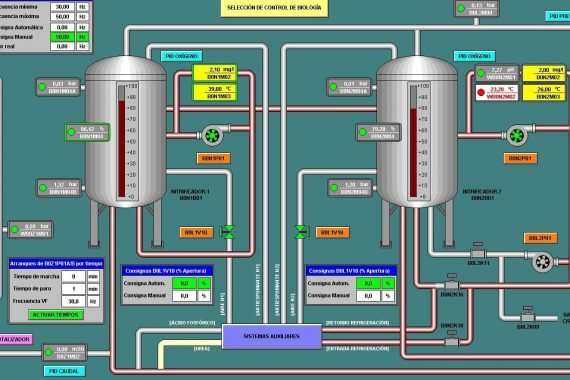
\includegraphics{Supervisorio_exemplo}
	\caption[Fonte: https://www.agaads.com/service/scada-system/]{Tela exemplo de um sistema supervisório}
	\label{img_supervisorio_exemplo}
\end{figure}

Os dados adquiridos podem ser manipulados de modo a gerar valores para parâmetros de  controle  como “set-points”. Os  dados são  armazenados em  arquivos de dados padronizados, ou apenas utilizados para realização de uma tarefa. Esses dados que foram armazenados em arquivos poderão ser acessados por programas de usuários para realização de cálculos, alteração de parâmetros e de seus próprios valores. (MACHADO MARTINS, 2012).

Outro emprego comum de sistemas SCADA, é de serem responsáveis por informar valores de setpoint aos controladores acoplados a um processo, os quais podem advir de um cálculo computacional ou manualmente, por um operador. É possível ainda o sistema ser responsável pelo controle, enviando aos atuadores conectados somente o sinal de controle. Esta estratégia, no entanto, não é recomendada, por questões de confiabilidade da transmissão de dados e velocidade de processamento.

Por ser executado geralmente em um computador comum, a palavra chave de um sistema supervisório é flexibilidade. Um sistema SCADA deve ser capaz de se comunicar por diversos protocolos com diversos dispositivos, e adicionalmente disponibilizar os valores lidos para outros usuários, não somente os que têm acesso às telas. Por possuir esta funcionalidade, software SCADAs ultrapassam o nível 2 na pirâmide de automação, referente à supervisão e controle de uma célula específica de produção, chegando ao nível seguinte, de supervisão da produção, pois agrupa as informações de diversos controladores e sensores em um só local, gerando suporte para ações de gerência.

\begin{figure}
	\centering
	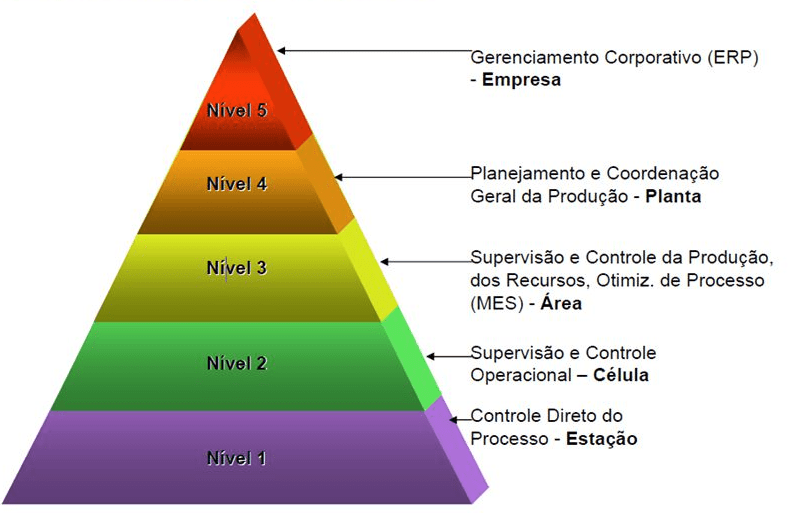
\includegraphics{piramide_automacao}
	\caption{Pirâmide da automação}
	\label{img_piramide_automacao}
\end{figure}

A fim de atingir uma maior compatibilidade com programas e usuários externos, a maior parte dos softwares supervisórios permitem de forma simples a criação de um banco de dados para os valores monitorados. Os mesmos podem ser exportados em forma de relatórios em layouts já embutidos e utilizados como insumos para tomada de decisões e cálculo de performance.

Segundo Leandro, et al, dentre os principais benefícios do uso de sistemas de supervisão podem-se citar: informações instantâneas, redução no tempo de produção, redução no custo de produção, precisão das informações, detecção de falhas, aumento da qualidade e aumento da produtividade.

\section{Comunicação Serial}

Comunicação serial é um meio simples de dois equipamentos trocarem informação em formato de uma série de bits. Ela ocorre através de um único cabo ou pino em um circuito integrado, sendo este um dos motivos da sua popularidade: o baixo custo necessário para a montagem da infraestrutura. A desvantagem disto é a perda em velocidade, pois transmite-se apenas um bit de cada vez, enquanto que existem tecnologias, como a chamada comunicação paralela, que utilizam mais canais de comunicação e podem transmitir vários bits simultaneamente.

Diversos equipamentos eletrônicos utilizam a comunicação serial, como mouses e teclados. O conhecido controlador Arduino UNO também permite a troca de bits por meio de uma porta serial. Ela também está presente em alguns protocolos de comunicação modernos, como Ethernet e Profibus.

Um modelo de transmissão para um byte (8 bits) de informação por porta serial se constitui em uma onda digital cujos formato se traduz em um bits 1 ou 0. O primeiro bit marca o início da transmissão, seguido por 8 bits relativos à informação enviada, um bit opcional de paridade (que torna o dados mais confiáveis), e um último bit que encerra o bloco de informação. Protocolos de comunicação diferentes podem acrescentar ou remover características à sequência transmitida, seja para assegurar a integridade dos dados ou para aumentar a velocidade de comunicação.

\begin{figure}
	\centering
	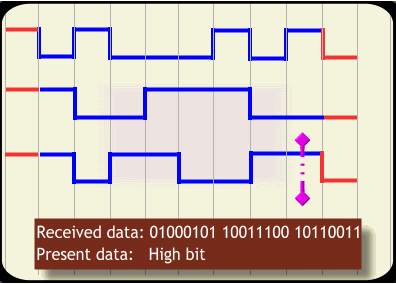
\includegraphics{serial_comm}
	\caption{Exemplo de transmissão serial de uma sequência de 3 bytes}
	\label{img_serial_comm}
\end{figure}

Por comunicar dois equipamentos distintos, com diferentes arquiteturas, se fazem necessárias medidas que contornam a diferença entre os clocks de ambos, em outras palavras, a diferença entre a velocidade de transmissão e a de leitura dos bits recebidos. Uma delas é a utilização de um buffer, um espaço de memória na porta receptora, que guarde rapidamente os bits transmitidos, para posterior leitura e tratamento dos mesmos por parte do processador da máquina. Quando este buffer está próximo de encher, o receptor pode fechar o barramento serial via hardware ou software, para impedir a perda de informação durante sua transmissão.

\section{Qt em Python}

Com traços da linguagem C e Perl, Python foi criada por Guido van Rossum no início da década de 90. É uma linguagem de alto nível, orientada a objetos e com tipagem dinâmica e forte. As definições de escopo e blocos de código são representadas por indentações, o que torna o código mais organizado e visualmente aprazível. Além disto permite interoperabilidade com outras linguagens. Por exemplo, utilizando a ferramenta Cython é possível, a partir de um código Python, gerar um código equivalente em C. Existem funções, inclusive, que são desenvolvidas em C, a fim de agilizar o processamento de grandes bases de dados, mas implementadas em Python.

No âmbito acadêmico, Python apresenta boas vantagens. Não só é considerada simples fácil de aprender, como é gratuita e open source. Logo, seus usuários e clientes não têm custos com licenças e seus desenvolvedores podem usar livremente códigos publicados por terceiros, que geralmente se apresentam de fácil acesso na internet, e adaptá-los às suas necessidades. Em uma enquete realizada pelo conhecido fórum da comunidade de computação Stack Overflow, Python foi considerada a 3ª “linguagem mais amada” pelo público.

Pela facilidade de compartilhamento e comunidade crescente, existem diversas bibliotecas de Python que podem ser baixadas com o simples comando no terminal pip install, configurado na instalação da linguagem. Como alguns exemplo, cita-se as libs SQLAlchemy, que permite criação e acesso a bancos de dados leves; NumPy, uma poderosa ferramenta para cálculos matriciais; e PyQt5, que possui objetos gráficos e métodos para criação de interfaces gráficas.

A biblioteca PyQt5 veio da biblioteca de C++ “Qt”, que implementa APIs para outras linguagens. No seu site oficial, existe uma documentação extensa de todos os seus objetos em C++, e existem também muitos exemplos disponíveis online, tanto em sites oficiais do Qt como em fóruns de programadores.

Existem 3 módulos do PyQt julgados principais para criação de GUIs locais:

\begin{itemize}
	\item QtWidgets: Engloba os objetos gráficos principais, como botões, textos e layouts. O objeto genérico QWidget, herdado por diversos outros deste módulo, tem funções cruciais relativas ao posicionamento, geometria, visibilidade e estilo dos objetos gráficos.
	\item QtCore: Este módulo lida com eventos dos objetos da GUI, como cliques de botões e edições de caixas de texto, e conecta estes eventos com funções definidas pelo programador. Ele também permite que ele configure a aplicação principal e coordena possíveis threads iniciadas por ela.
	\item QtGui: Contém objetos que possibilitam a edição de cores e bordas dos Widgets e também lida com eventos relacionados à atualização da posição e estética destes objetos.
\end{itemize}

Para iniciar a GUI, deve ser criado um objeto \emph{QApplication}, que representa o núcleo da aplicação, juntamente com as janelas da mesma, que são objetos \emph{QMainWindow}. Estes aceitam um objeto \emph{QWidget} como Widget central principal (através do método \emph{setCentralWidget()}), cujas características de tamanho e layouts internos definem o tamanho da janela. Inicia-se a aplicação pelo comando \emph{exec\_()}, e as janelas pelo comando \emph{show()}.

Numa interface criada com PyQt5, os objetos visíveis dispostos na tela são chamado de Widgets. Como dito, a maioria herda direta ou indiretamente do objeto \emph{QWidget}. Por conta da arquitetura da biblioteca, uma boa prática para programadores é colocar um Widget dentro do outro, no sentido de design e posicionamento. Assim, é possível definir melhor o espaço e as condições de redimensionamento dos objetos quando a janela for esticada ou comprimida.
No apêndice deste documento, se encontra um pequeno guia de como criar aplicações com PyQt5, elaborado pelo autor.

\begin{figure}
\centering
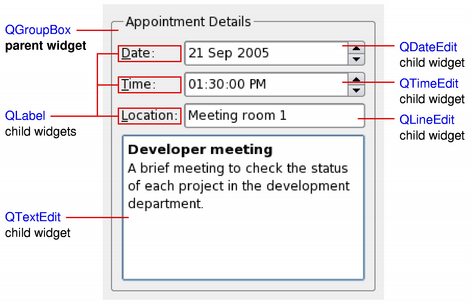
\includegraphics{Exemplo_QWidget}
\caption{Janela \emph{QMainWindow} com um \emph{QGroupBox} como Widget central, contendo vários outros Widgets em um layout \emph{QGridLayout} dentro de outro layout \emph{QHBoxLayout}}
\label{img_exemplo_qwidget}
\end{figure}

\chapter{Desenvolvimento do Sistema Supervisório}

\section{Requisitos do Sistema}

Para a escolha da tecnologia empregada, foram levantados os seguintes requisitos do sistema:
\begin{itemize}
	\item Deve ser gratuito para o desenvolvimento, simples e de código aberto no intuito de permitir análise por partes de interessados e facilitar melhorias e expansões;
	\item Deve ser capaz de desenhar gráficos em tempo real, advindos de porta serial. Opcionalmente pode ser compatível com arquivos nos formatos .csv, .tsv, .xls, e .xlsx, ou permitir modelagem direta no \textit{software}, por funções de transferência
	\item O \textit{software} deve rodar no sistema operacional windows (mínimo Windows 7)
\end{itemize}

\section{Seleção das Tecnologias}

Pelo primeiro requisito, em relação à gratuidade da tecnologia, pensou-se primeiramente em utilizar plataformas abertas para sistemas supervisórios, como o ScadaBR ou a versão demo do Elipse E3. Já houveram trabalhos, inclusive, utilizando a primeira tecnologia \cite{Moraes2016}.

Como atestado em \citeonline{Moraes2016}, o ScadaBR é construído em um servidor web, utilizando geralmente o Apache TomCat (como servidor web). É um \emph{software} \emph{open source} e existem vários materiais \emph{online}, tanto escritos como em vídeo orientando interessados em como utilizá-lo. Porém, os protocolos de comunicação pré-configurados são Modbus (IP e Serial) e OPC. Para aplicações com arduino, o usuário teria que criar uma função que enviasse os dados ao sistema no formato correto.

Quanto à versão demo do Elipse E3, segundo \citeonline{Elipse2019}, permite somente até 20 tags de dados e a aplicação roda por um máximo de 2 horas, tendo que ser reiniciada manualmente após este período. Isto a torna uma ferramenta muito limitada. Adicionalmente, não se sabe as implicações legislativas em utilizar o \emph{software} para trabalhos acadêmicos, nem sua utilização contínua no âmbito da universidade, mesmo se tratando de uma versão de demonstração.

Por cumprir todos os requisitos, e por ser considerado um método mais facilmente escalável, em questão de tecnologias atuais, foi decidido construir um sistema SCADA em Python. Desta maneira, o código-fonte da aplicação seria aberto, compatível com diferentes sistemas operacionais, e este trabalho contribuiria na difusão da implementação de \textit{software} gratuitos e \textit{open source} no meio acadêmico. Além disto, Python é uma linguagem contemporânea, tendendo a acompanhar o avanço tecnológico. Desta forma, o sistema desenvolvido seria compatível com uma vasta gama de tecnologias modernas, como por exemplo, armazenamento em nuvem.

\subsection{Seleção das bibliotecas}

Como já mencionado, a linguagem Python possui inúmeras bibliotecas, para os mais variados fins. No decorrer da criação do sistema, foram utilizadas as seguintes bibliotecas no Quadro \ref{qdr_used_libs}.

\begin{quadro}
	\centering
	\caption{Bibliotecas Python utilizadas no desenvolvimento do supervisório didático}
	\begin{tabular}{|m{5em}|m{25em}|}
		\hline
		Biblioteca & Descrição \\
		\hline
		PyQt5 & Usada para a construção de GUIs, contém diversos objetos úteis como botões, caixas de texto e rótulos. Também trata do posicionamento e direção destes objeto nas janelas principal e periféricas \cite{pyqtdoc} \\
		\hline
		PyQtChart & Conjunto de conectores de python para a biblioteca Qt \\
		\hline
		matplotlib & Contém ferramentas que permitem o desenho e design de gráficos variados, inclusive com objetos backend que fazem uma ponte com GUIs construídas com PyQt5 \cite{hunter2007matplotlib} \\
		\hline
		numpy & Biblioteca que lida com operações matriciais e cálculos avançados, com muitas funcionalidades similares ao MatLab. Também é capaz de gerar números aleatórios, que são úteis no teste do programa \cite{harris2020array} \\
		\hline
		pyserial & Permite a conexão com dispositivos externos pela porta serial e contém funções de escrita e leitura desta porta \cite{pyserial} \\
		\hline
		python-control & Possibilita a criação de sistemas descritos em funções de transferência e espaço de estados, além de gerar a resposta simuladas para alguns formatos comuns de entradas, como degrau e impulso \cite{pythoncontrol} \\
		\hline
		pickle & Responsável pera serialização de objetos utilizados no código e armazenamento dos mesmos em um arquivo à parte. Lida também com a leitura e decodificação de objetos serializados \\
		\hline
	\end{tabular}
	\label{qdr_used_libs}
\end{quadro}

\section{A interface gráfica}

A biblioteca PyQt funciona como uma linguagem orientada a objetos. Assim, esta arquitetura foi adotada no desenvolvimento da ferramenta. Foi utilizado uma folha de \emph{script} que agrupasse a maior parte das classes implementadas, o form\_objects.py, e outro \emph{script} principal, main.py que inicia a execução do programa. Um terceiro \emph{script}, realtime\_objects.py, contempla objetos que rodam em tempo real e espera-se que futuros usuários também editem o código contido, por motivos explanados posteriormente neste documento. No Apêndice \ref{Chap:Apendice1} encontra-se um tutorial de utilização do supervisório.

No que concerne a interface gráfica do supervisório, imaginou-se um \emph{layout} simplista. A aplicação conteria uma área para apresentação de gráficos, uma lista das séries de dados incluídas no programa pelos diversos métodos possíveis, e uma área para incluir séries novas. Os detalhes destes Widgets são listados abaixo, e sua disposição mostradas na Figura \ref{img_gui_macro}:

\begin{itemize}
	\item \emph{PlotManager}: representaria uma área de rolagem (QScrollArea) que conteria várias representações gráficas das séries de dados salvos na aplicação, com uma pequena \emph{preview} destes dados, e botões para seu desenho, edição e exclusão da série.
	\item \emph{MainPlotArea}: utiliza um objeto \emph{FigureCanvas}, da lib matplotlib, para criação de um gráfico detalhado das séries selecionadas na lista de séries. O eixo y assumiria várias dimensões, a depender da variável representada, e o eixo x englobaria o tempo.
	\item \emph{DatasetConfig}: tem como Widget principal um seletor com abas (\emph{QTabWidget}), que permitiria a inclusão de séries de dados novas no programa, pelas fontes já mencionadas, sendo cada aba responsável pelas diferentes métodos (serial, arquivo, função de transferência, etc)
	\item \emph{SCADADialog}: se trata realmente de uma tela de supervisão, com uma área de gráficos atualizada em tempo real. Funciona somente quando os dados são importados por porta serial.
\end{itemize}

\begin{figure}[hbt]
	\centering
	\caption{Supervisório didático e seus objetos principais}
	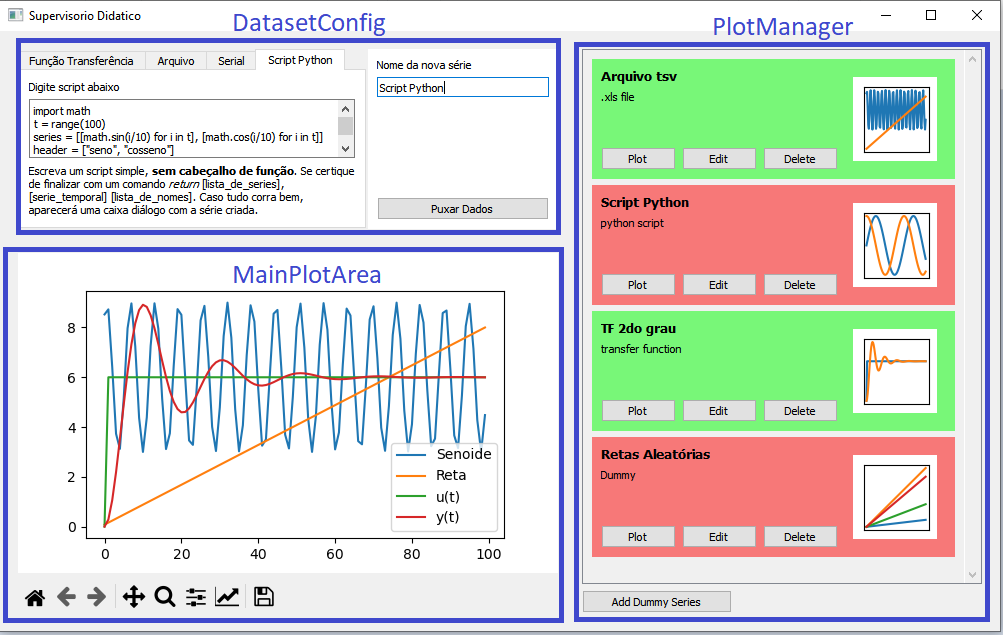
\includegraphics[width=\textwidth]{GUI_macro}
	\label{img_gui_macro}
\end{figure}

Além dos Widgets supracitados, para simplificar o código e torná-lo mais prático, foi criado um objeto abstrato \emph{SeriesObject}. Ele armazena um agrupamento de série de dados que compartilham um mesmo eixo de tempo. Desta forma, foi mais fácil manipular as referências das séries pelo programa. Uma imagem contendo todos os objetos criados no desenvolvimento do programa, bem como suas relações e funções, encontra-se no Apêndice \ref{Chap:Apendice2}.

\section{\emph{Dataset Config}}

A principal função deste objeto é de interface da aplicação com outros dispositivos ou programas, com a finalidade de puxar séries de dados destas fontes. A segunda função é de formatar estas séries, atribuindo a elas um nome e um cabeçalho, além de definir que legenda aparece no gráfico principal quando ele for desenhado.

Na fase de idealização do \emph{software}, levantou-se possíveis meios para adicionar séries de dados novas no programa. Como se trata de um sistema supervisório, deve haver uma funcionalidade que permita o recebimento de dados externos, no mínimo por comunicação serial, bastante utilizada por controladores didáticos como Arduino e Raspberry Pi. Como adicionais,, seria útil também a importação de séries por arquivos \emph{.xls} ou \emph{.xlsx}. Por último, caso o usuário deseje utilizar funcionalidades não ofertadas pelo \textit{software} didático, ele pode escrever seu próprio script Python e levar os resultados para o programa.

Como o supervisório foi desenvolvido para a área didática da automação, ele deveria oferecer uma maneira simples de simular processos diversos e representar as simulações por gráficos, contrastando-as com o sistema real, proveniente do controlador. Logo, foi incluída biblioteca que simulasse as resposta de funções de transferência, por padrão a uma entrada degrau, e fornecidos os meios para que o usuário encadeie em série variadas funções, de parâmetros quaisquer, pelo objeto \emph{TransferFunctionConfig}.

Resumindo, existem quatro maneiras de importar ou gerar uma série de dados no \emph{software} desenvolvido:

\begin{enumerate}
	\item \textbf{Por arquivo}, nos formatos \emph{csv} (Comma Separated Values), \emph{tsv} (Tab Separated Values), \emph{xls} (antigo arquivo Excel), \emph{xlsx} (arquivo Excel);
	\item \textbf{Por função de transferência}, informando o numerador e denominador de cada função, criadas em série e submetidas a uma entrada do tipo degrau, de valor definido pelo usuário;
	\item \textbf{Por comunicação serial}, configurando alguns parâmetros (porta, baud rate e tempo para timeout), separando cada valor enviado pelo dispositivo por uma tabulação e linhas por quebras de linha;
	\item \textbf{Por script Python}, escrevendo um código python funcional e retornando os valores das séries na ordem correta (lista dos valores das séries, série de valores de tempo, lista de nomes das séries, nesta ordem)
\end{enumerate}

Caso não haja problemas na importação e as condições de formatação para cada método de entrada forem satisfeitas, o programa abrirá uma caixa diálogo (\emph{QtWidgets.QDialog}) idêntica à da Figura \ref{img_edit_series_dialog} com uma \textit{preview} dos dados e uma tabela com os valores numéricos. Através dele é possível editar cada valor separadamente, o nome da série e o cabeçalho.

\begin{figure}[hbt]
	\centering
	\caption{\emph{ModelSeriesDialog}: Caixa diálogo para edição dos eixos e título das séries}
	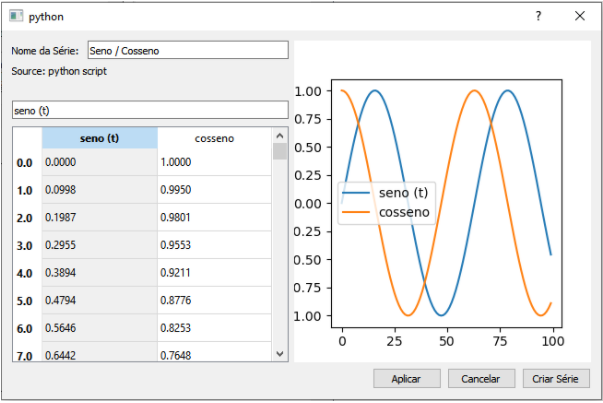
\includegraphics[width=\textwidth]{edit_series_dialog}
	\label{img_edit_series_dialog}
\end{figure}

Esta caixa diálogo contém um Widget frequentemente utilizado na aplicação: o \emph{FigureCanvas}, proveniente de um módulo da biblioteca matplotlib, que funciona como um plugin para o PyQt. Apesar dele não ser um Widget do PyQt, ele contém, se não todos, uma boa parte de seus módulos e é tratado como tal para fins de posicionamento, geometria e inclusão nos \textit{layouts} de tela. O \emph{FigureCanvas} faz uma interface com o objeto \emph{Figure}, responsável pela criação de gráficos de linhas, barras, etc, e permite que ele seja incluído numa GUI construída em PyQt.

O objeto \emph{Figure}, por sua vez, é bem similar ao objeto de mesmo nome no MATLab\textsuperscript{\tiny \textregistered}, aceitando métodos como \emph{plot()}, emph{add\_subplot()} e \emph{clear()}. Sua documentação completa, juntamente com a de outros objetos relevantes consta no site da biblioteca \href{https://matplotlib.org/}{matplotlib}. Quando embutido numa GUI por um \emph{FigureCanvas}, após o desenho de gráficos e de formatações gerais, o segundo deve chamar o método \emph{draw()} para que seja atualizada a imagem.

%\textcolor{red}{Devo Focar no algoritmo de cada tipo de importação??}

\section{\emph{PlotManager}}

Como consta na Figura \ref{img_gui_macro} o lado direito da aplicação, se encontra uma lista das séries carregadas. Dado o espaço limitado, faz-se necessária uma área de rolagem. Assim, foi criado um objeto \emph{GraphicPlotList} que implementa esta área ao herdar de \emph{QtWidgets.QScrollArea}.

Quando uma série nova é criada pelo \emph{DatasetConfig}, ela fica armazenada em um objeto \emph{SeriesObject}, que é representado graficamente na lista de séries \emph{GraphicPlotList} por um outro objeto \emph{GraphicPlotConfig} (Figura \ref{img_graphic_plot_config}).

\begin{figure}[hbt]
	\centering
	\caption{\emph{GraphicPlotConfig} não desenhado em \emph{MainPlotArea}}
	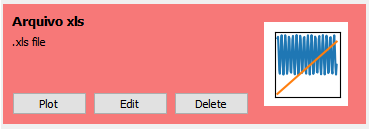
\includegraphics{graphic_plot_config}
	\label{img_graphic_plot_config}
\end{figure}

A principal função deste objeto é identificar pelo nome e fonte a série que contém, e coordenar quando esta série deve ser desenhada na área principal \emph{MainPlotArea}, além de permitir sua edição ou deleção. Contribuindo com a identificação dos dados, foi incluída uma visualização simples das séries, o que torna o visual estético. A cor de fundo do \emph{GraphicPlotConfig} alterna entre verde e vermelho, indicando se as séries contidas foram desenhadas ou não. Ao clicar no botão “Edit”, uma caixa diálogo idêntica à de incluir uma série nova aparece permitindo que o usuário edite seus valores, cabeçalho e nome.

Em PyQt, os objetos de uma GUI são “pintados” na tela por um objeto \emph{QtGui.QPainter}, de acordo com sua área, e paleta de cores. A primeira informação depende de alguns parâmetros, como o \textit{layout} no qual ele está inserido ou sua política de tamanho (QSizePolicy). Isto ocorre no método \emph{paintEvent(event)}, chamado automaticamente quando o objeto é reposicionado ou quando sua aparência deve ser atualizada (cada caractere novo digitado numa caixa de texto, por exemplo).

Essa dinâmica torna necessário que o método seja sobrecarregado quando o programador deseje customizar a aparência de um botão ou o seu plano de fundo. A desvantagem é que, por sobrecarregar o método que pinta o objeto na interface, o objeto deve ser repintado manualmente. No caso de um botão, por exemplo, no mínimo o método \emph{drawRectangle()} e \emph{drawText()} deve ser invocado. Assim, quanto mais detalhado for um objeto, mais complicado se torna alterar suas cores e formatos internos. Existem maneiras que contornam a necessidade de criar um novo objeto e sobrescrever o método \emph{paintEvent()}, utilizando as chamadas stylesheets. Porém, para este trabalho, julgou-se mais simples a primeira opção, pelo fato dos objetos customizados possuírem um design pouco complexo.

O objeto \emph{GraphicPlotConfig}, por alternar suas cores de fundo, teve seu evento de "pintura" sobrecarregado. Como sua tela de fundo é representada apenas por um retângulo, sua implementação não foi muito dificultosa.

\section{\emph{MainPlotArea}}

Se tratando de análises de sistemas, a visualização dos dados é essencial. No canto inferior esquerdo da GUI, existe uma área de gráficos, implementada por um objeto \emph{FigureCanvas} (Figura \ref{img_main_plot_area}. Abaixo dele, uma faixa de ferramentas (\emph{NavigationToolbar2QT}) permite que o usuário edite algumas propriedades do gráfico gerado, aproxime ou distancie a imagem e, principalmente, salve a figura em formato de imagem. Na lista de séries à direita, ao clicar no botão “Plot”, a série associada serão desenhadas no Canvas, com legenda.

\begin{figure}[htb]
	\centering
	\caption{\emph{MainPlotArea}}
	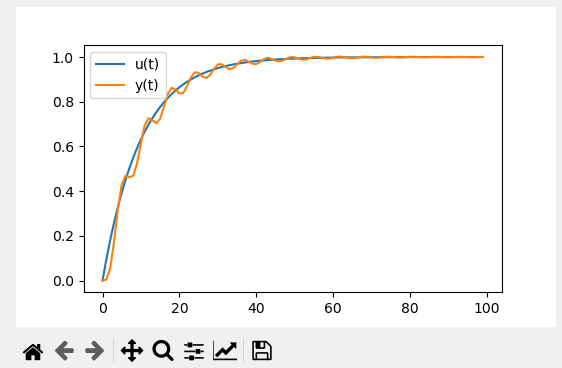
\includegraphics[width=0.8\textwidth]{main_plot_area}
	\label{img_main_plot_area}
\end{figure}

\section{\emph{SCADADialog}}

Um sistema supervisório, como o apresentado neste documento, monitora dados de controladores geralmente industriais em tempo real. Por se tratar de um \emph{software} didático, foi incluído no programa um suporte para futuras comunicações com um Arduíno ou qualquer outro microcontrolador ou até mesmo dispositivos que permitam comunicação serial. Assim, configurados os parâmetros de comunicação (\emph{baud rate}, nome da porta e tempo de timeout), o usuário pode visualizar graficamente dados enviados por um controlador em tempo real, desde que os mesmos estejam no formato esperado: tabulações para separar diferentes séries de dados e quebras de linhas para finalizar um registro.

Ao importar dados por fonte serial no \emph{DatasetConfig}, sugere-se sempre testar a comunicação antes de clicar no botão “Puxar dados”. quando o mesmo é clicado, uma caixa diálogo \emph{DialogHeader} é aberta, para que o usuário edite os nomes das variáveis recebidas via serial. A primeira série é sempre o tempo, e o dispositivo conectado \textbf{deve} obedecer esta ordem. Ao clicar em OK nesta caixa, a comunicação com a porta serial será iniciada e uma janela de monitoramento surgirá, caso não tenha ocorrido nenhum erro de comunicação.

%Vale a pena colocar referencia nestes trechos?
O código da comunicação com periféricos implementa duas \emph{threads} da biblioteca nativa \emph{\_thread} do Python. Segundo \citeonline{threads}, threads são trechos de código que rodam simultaneamente em um mesmo processo pai. Por conta disso, ao utilizar esta estrutura, alguns cuidados devem ser tomados pelo programador, no que se refere a acesso compartilhado à memória. Como não há controle de execução de cada thread separadamente, bugs podem ocorrer caso mais de um processo acesse e modifique o mesmo objeto ou variável simultaneamente.

Para contornar este problema, existem algumas estruturas que controlam o acesso de memória em programas que implementam threads, como monitores e semáforos. O último é, talvez, o mais trivial. Um semáforo possui dois estados: aberto ou fechado. Quando uma thread toma controle de um objeto no código, o semáforo é fechado, impedindo que outras threads façam o mesmo, até que o objeto seja liberado e o semáforo reaberto. Para Python, existem bibliotecas que implementam estruturas de controle, como a \emph{asyncio}, porém, por ser uma estrutura simples e não utilizada mais que algumas vezes no código-fonte deste trabalho, uma variável booleana bastou.

Após a conexão bem sucedida com o dispositivo, o programa escreve uma mensagem na porta serial (“go”, por padrão) e inicia suas duas threads, uma para ler dados da porta, e outra para atualizar o Canvas da caixa diálogo \emph{SCADADialog}. Esta separação se fez necessária pois o método do Canvas que o atualiza (emph{draw()}) é considerado custoso, e poderia travar a aplicação se fosse executada repetidas vezes. Outro motivo para implementação das threads é exemplificar a estudantes do código uma implementação simples de paralelismo, o que pode ser bastante util e que não é abordadas nos cursos tradicionais de Engenharia (excetuando computação).

Cada uma das threads tem um tempo de repetição, que define a periodicidade que elas executam suas instruções. O padrão definido foi de 0,1 segundos para ler dados da porta serial, e 1 segundo para atualizar o gráfico com os valores lidos. Quando a leitura da porta ocorre, os valores são armazenados em uma lista compartilhada. Quando a rotina de atualização é chamada, os valores desta lista são movidos para outra, chamada \emph{plotted}, que por sua vez gera um gráfico, e o Canvas é atualizado. A manipulação de uma lista compartilhada justifica o emprego de um semáforo, pois uma \textit{thread} escreve nesta lista e outra a lê.

Como já mencionado, o programa espera que os dados recebidos sejam espaçados por tabulações, separando diferentes variáveis, e quebras de linhas, separando diferentes leituras ao longo do tempo de execução. O primeiro valor lido sempre é considerado o tempo, e deve vir do dispositivo conectado, pois o mesmo é quem dita o andamento do processo controlado. Caso o número de variáveis numa mesma linha lida seja diferente do configurado no objeto DatasetConfig, o programa considerará que houve um erro e toda a linha de dados será ignorada.

A figura \ref{img_esquema_serial} esquematiza a execução do código de monitoramento serial:

\begin{figure}[hbt]
	\centering
	\caption{Esquema de leitura serial no supervisório didático}
	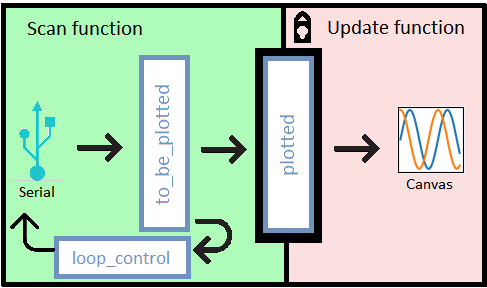
\includegraphics{esquema_serial}
	\label{img_esquema_serial}
\end{figure}

Para que o programa possa ser de fato implementado em aulas, foram adicionadas duas funções que possibilitam de envio de dados ao dispositivo conectado a cada leitura da porta serial. Isto seria uma analogia a um controlador que atuasse num processo físico, medido por tal dispostivo. Desta forma, o último simularia o sistema em si, enquanto que parte do supervisório didático assumiria o papel de controlador. Devido à popularidade do microcontrolador Arduino, a implementação da rotina de controle dentro do \emph{software} foi projetada similarmente à sua programação. A rotina é feita em duas etapas, uma na função \emph{setup\_control}, chamada logo após uma conexão bem-sucedida com o dispisitivo, uma única vez, e outra na função \emph{loop\_control}, chamada logo após cada leitura da porta serial.

Numa aplicação de controle PID, por exemplo, a primeira função realizaria sua sintonia ou informaria à "planta" os parâmetros de seus processos, enquanto que a segunda função receberia do supervisório a última linha lida da porta, calcularia a resposta do controlador PID, e escreveria o resultado de volta. Obviamente, o dispositivo conectado deve ser programado para receber esta informação, o que requer certo conhecimento do usuário, tanto de Python como do dispositivo em si. Felizmente, códigos de exemplo se encontram disponíveis neste documento.

Durante o monitoramento e registro dos valores trazidos via serial, o gráfico irá atualizar numa janela de 20 segundos, contando do maior tempo registrado para trás. Isto se justifica no comportamento dinâmico da maioria dos sistemas, que atinge valores por vezes maiores que os estacionários. Esta medida impede que a escala do gráfico fique prejudicada, e variações pequenas relativas a um comportamento estacionário não sejam bem percebidas. O usuário pode, de todo modo, em tempo de execução clicar nos botões “Parar” e “Criar Série”, salvar as séries de dados lidas e desenha-as no objeto MainPlotArea, visualizando todo seu comportamento histórico.

\section{Salvamento Automático de Séries}

Durante a utilização do supervisório didático, espera-se que ajustes sejam feitos nas funções que simulam o controlador. Quando o script Pyhton é iniciado, uma cópia dele é criada e compilada, tornando impossível que alterações no script original em tempo de execução tenham influências no sistema. Por isso, o usuário tem que fechar o supervisório didático sempre que desejar alterar as funções \emph{setup\_control()} e \emph{loop\_control()}, o que resultaria na perda das séries já salvas pelo programa.

Para amenizar este problema, foi incluída uma funcionalidade de salvamento automático na aplicação. Uma das bibliotecas nativas do Python, o \emph{Pickle}, permite que um objeto ou variável do programa seja serializada em formato de arquivo, e salva em um diretório no computador. Isto ocorre através do comando \emph{pickle.dump()} Desta forma, o arquivo pode ser restaurado (\emph{pickle.load()}) e reincorporado ao código com os mesmos valores de atributos que possuía quando foi serializado.

Sempre que uma série é incluída, editada ou deletada, o arquivo "autosave.dat" é sobrescrito com a lista de séries da sessão (\emph{listSeries}). Em contrapartida, quando o objeto \emph{PlotManager} é inicializado, o arquivo "autosave.dat" é aberto e a lista de séries lá salva é restaurada.
\chapter{Caso de Teste}

\section{Apresentação do Sistema}

Para ilustrar o funcionamento do sistema supervisório, foi utilizado um Arduino UNO que simulasse o funcionamento de um processo com dois tanques de área variável acoplados. A Figura abaixo o esquematiza:

\begin{figure}[H]
	\centering
	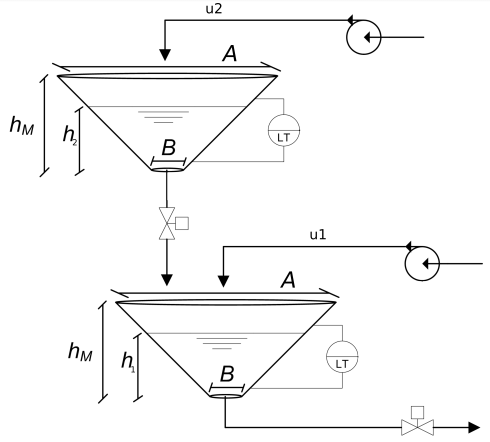
\includegraphics[width=0.8\textwidth,height=0.4\textheight]{sistema_teste}
	\caption{Esquema de leitura serial no supervisório didático\\Fonte: Elaborado pelo Prof. Daniel Santana}
	\label{img_sistema_teste}
\end{figure}

Como percebido pelo esquema, os tanques têm o formato de tronco de cone e a variável controlada é a sua altura. O controle é feito por 2 bombas que aumentam ou diminuem a vazão de entrada de fluido em ambos os tanques. A medição é realizada por dois sensores de nível, sujeito a ruídos brancos.

As equações deste processo são descritas abaixo:
\\\\
$
\frac{dh_1}{dt} = \frac{1}{\beta(h_1)}(u_1 - k\sqrt{\rho g h_1} + k\sqrt{\rho g h_2})\\
\frac{dh_2}{dt} = \frac{1}{\beta(h_2)}(u_2 - k\sqrt{\rho g h_2})\\
\beta(h_i) = \frac{dV}{dh_i}\\
V(h_i) = \frac{\pi\gamma^2}{3}(h_i + \frac{B}{2\gamma})^3 - \frac{\pi}{3\gamma}(\frac{B}{2})^3\\
\gamma = \frac{A-B}{2h_M}\\
$

Seus parâmetros e variáveis são descritos e dimensionados na tabela \ref{tbl_parameters}:

\begin{table}[H]
	\centering
	\begin{tabular} {|m{5em}|m{15em}|m{8em}|}
		\hline
		Símbolo & Descrição & Valor (u.m.) \\
		\hline
		A & diâmetro superior & 4 ($m$) \\
		B & diâmetro inferior & 1 ($m$) \\
		hm & altura máxima & 4 ($m$) \\
		V & volume & - ($m^3$) \\
		h & altura & - (m) \\
		$\rho$ & densidade do fluido & 1000 ($kg/m^3$) \\
		g & aceleração da gravidade & 9,8 ($m/s^2$) \\
		k & constante de descarga no tanque & 0,001 (-)\\
		u & vazão da bomba & - ($m^3/s$)\\
		\hline
	\end{tabular}
	\caption{Tabela de parâmetros e variáveis do sistema}
	\label{tbl_parameters}
\end{table}

\section{Comportamento esperado}[\label{comportamento_esperado}]

Por se tratar de um sistema não linear, pouco pode-se dizer de seu comportamento dinâmico, partindo-se somente das esquações. Porém, é possível prever possíveis estados estacionários, onde a taxa de variação dos estados no tempo é nula.

Com as derivadas zeradas nas equções descritivas, tem-se:
\\\\
$
{h_1}_{ss} = (\frac{{u_1}_{ss}}{k\sqrt{\rho g}} + \sqrt{{h_2}_{ss}})^2
$
\\
$
{h_2}_{ss} = \frac{{u_2}_{ss}^2}{k^2 \rho g}
$
\\
Como os estados estacionários são reais e finitos, o sistema é dito estável. Nota-se também que, caso a bomba 1 seja desligada, é possível manter as alturas em um ponto diferente de zero somente com a acão da bomba 2, e ambas assumirão os mesmos valores (${h_1}_{ss} = {h_1}_{ss}$).

\section{Sintonia do Controlador}

Por tratar-se de um sistema não linear, serão comparados dois controladores sintonizados por métodos distintos. No primeiro caso, o sistema será linearizado em torno de um ponto de operação e o resultado será utilizado para sintonizar um controlador PID. Em seguida o controlador será acoplado ao sistema. No segundo caso, será utilizada uma lei de controle que anula a não-linearidade do sistema, transformando-o em uma sistema linear. Após este passo, também será utilizado um controlador PID para controlá-lo.

\subsection{Linearização do Sistema}

O processo de linearização de um sistema consiste na aplicação da série de Taylor em suas equações descritivas num determinado ponto de operação.

\begin{figure}[H]
	\centering
	$
	f(x1, x2, .. , xn) \simeq f(x1_0, x2_0, ..., x3_0) + \bigg( \sum_{i=1}^n \frac{df}{dxi}\big|_{xi=xi_0} (xi - xi_0) \bigg)
	$
	\caption{Série de Taylor truncada na primeira ordem}
\end{figure}

sendo a expressão $(xi - xi_0)$ chamada de desvio e representada por $\overline{xi}$.

Aplicando a linearização no sistema de estudo, as novas equações do sistema, em desvio, serão então:
\\\\
$
\frac{dh_1}{dt} = -\big(\frac{d\beta^{-1}(h)}{dh}\bigg|_{{h_1}_{ss}} k\sqrt{\rho g {h_1}_{ss}} + \frac{\beta^-1({h_1}_{ss}) k\sqrt{\rho g}}{2\sqrt{{h_1}_{ss}}}\big)\overline{h_1} + \big(\frac{\beta^-1({h_1}_{ss}) k\sqrt{\rho g}}{2\sqrt{{h_2}_{ss}}}\big)\overline{h_2} +  \beta^{-1}({h_1}_{ss})\overline{u_1}
$
\\
$
\frac{dh_2}{dt} = -\big(\frac{d\beta^{-1}(h)}{dh}\bigg|_{{h_2}_{ss}} k\sqrt{\rho g {h_2}_{ss}} + \frac{\beta^-1({h_2}_{ss}) k\sqrt{\rho g}}{2\sqrt{{h_2}_{ss}}}\big)\overline{h_2} + \beta^{-1}({h_1}_{ss})\overline{u_2}
$
\\
$
\beta^{-1}(h) = \frac{4}{4\pi(\gamma h)^2 + 4B\gamma h + B^2} 
$
\\
$
\frac{d\beta^{-1}(h)}{dh} = -4 \frac{8 \pi \gamma^2 h + 4 \gamma B}{(4\pi(\gamma h)^2 + 4B\gamma h + B^2)^2}
$

De forma a zerar a função $\frac{dh_i}{dt}$ presente na série de Taylor, define-se como um bom ponto de operação um dos estados estacionários do sistema, como por exemplo,  $h_{1_0}=h_{1_{ss}}=1, h_{2_0}=h_{2_{ss}}=1, u_{1_0}=u_{1_{ss}}=0, u_{2_0}=u_{2_{ss}}=k\sqrt{\rho g}$. Substituídos os parâmetros de acordo com a tabela \ref{tbl_parameters} e em formato de espaço de estados o sistema final linearizado será
\\\\
$
\begin{pmatrix} \dot{\overline{h_1}} \\ \dot{\overline{h_2}} \end{pmatrix} = \begin{pmatrix} -0,063 & 0,046 \\ -0,063 & 0 \end{pmatrix} \begin{pmatrix} \overline{h_1} \\ \overline{h_2} \end{pmatrix} + \begin{pmatrix} 0,937 & 0 \\ 0 & 0,937 \end{pmatrix} \begin{pmatrix} \overline{u_1} \\ \overline{u_2} \end{pmatrix}
$
\\\\
\subsection{Sintonia do LQI}

\subsection{Sintonia do PI}

O controlador PI é um tipo bastante utilizado na indústria. Possui um ganho proporcional (P) e um ganho integrativo (I), que incidem sobre a diferença entre a medição atual de uma saída de processo e seu valor desejado. Isto exige que o sistema de controle seja realimentado com um valor geralmente advindo de um sensor, constituindo-o num sistema de malha fechada. A sintonia de um PI se traduz na definição de P e I, e pode ser realizada, entre outras formas, por métodos como Ziegler-Nichols, Coher-Coon ou até mesmo tentativa e erro.

Sendo $P(s)$ uma função de transferênciaentre a saída $Y$ de um processo e sua única entrada $u$, um método simples de sintonia, que dispensa experimentação é o chamado síntese direta.
Tomando um sistema em malha fechada representado na figura \ref{img_exemplo_processo}

\begin{figure}[H]
	\centering
	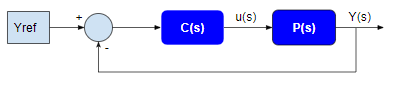
\includegraphics[width=0.8\textwidth]{exemplo_processo}
	\caption{Processo 1x1 com feedback e controlador}
	\label{img_exemplo_processo}
\end{figure}

sua função de tranferência entre a saída $Y$ e entrada $u$ será
\\\\
$
\frac{Y(s)}{u(s)} = \frac{C(s)P(s)}{1+P(s)C(s)}
$
\\

Desta forma, caso deseje-se modelar $Y(s)$ como uma função de primeiro grau $\frac{1}{\tau s + 1}$, a equação do controlador $C(s)$ assumirá
\\\\
$
C(s) = \frac{P^{-1}(s)}{\tau s}
$
\\

Caso $P$ seja uma função de primeiro grau, o controlador será um PI.

Para este método de sintonia, o cálculo dos ganhos do controlador de $h_1$ desconsidera a influência de $h_2$. Tomando como base o sistema linearizado e aplicando a equação da malha fechada, o mesmo será
\\\\
$
\overline{h_1}(s) = \frac{0,937}{s + 0,063} \overline{u_1}(s) + \frac{0,046}{s + 0,063} \overline{h_2}(s) 
$
\\
$
\overline{h_2}(s) = \frac{0,937}{s + 0,063} \overline{u_2}(s)
$
\\\\
logo, os controladores, projetados para um tempo de resposta $\tau$ de 10 segundos, serão:
\\\\
$
C_1(s) = C_2(s) = \frac{1}{10s} \frac{s + 0,063}{0,937} = 0,1067 + 0,0067 \frac{1}{s}
$

\section{Configuração do supervisório didático}

Como já mencionado, o programa apresentado implementa duas funções que podem ser editadas pelo usuário, de forma que seja possível uma resposta ao dispositivo conectado. O usuário pode ainda escrever suas próprias funções e alterar os objetos do código fonte como preferir, para atender as suas necessidades. 

\subsection{LQI}

\subsection{Controlador PI}

Além da biblioteca \emph{python-control}, existe outra chamada emph{simple-pid} que, como o nome indica possui objetos que se comportam como controladores PID. Eles recebem como parâmetrosseus respectivos ganhos, valor de referência da variável controlada, limites para a resposta e outros que são referenciados  \href{https://pypi.org/project/simple-pid/}{na página da biblioteca}. Para implementá-los no programa, na função \emph{setup\_control()}, criam-se tais objetos de acordo com o código abaixo:
\\\\
\texttt{\footnotesize self.pids = [] \\
	self.pids.append(simple\_pid.PID(0.1067, 0.0067, setpoint=2.5, output\_limits=(None, None))) \\
	self.pids.append(simple\_pid.PID(0.1067, 0.0067, setpoint=2.5, output\_limits=(None, None)))}
\\\\
O objeto PID, quando chamado, retorna um valor numérico referente à resposta do controlador a partir de uma leitura, informada como parâmetro. Este valor pode ser escrito na porta serial, e será capturado pelo dispositivo conectado, desde que o mesmo esteja preparado para recebê-lo. No Arduino, o comando \emph{\textbf{Serial}.parseFloat()} se mostrou satisfatório.

Implementando na função \emph{loop\_control()} a lógica descrita acima:
\\\\
\texttt{\footnotesize def loop\_control(self, input\_data): \\
	\hspace*{8mm}if len(input\_data) == 0: \\
	\hspace*{8mm}\hspace*{8mm} return \\\\
	\hspace*{8mm}signals = [self.pids[i](input\_value) for i, input\_value in enumerate(input\_data)] \\
	\hspace*{8mm}for signal in signals: \\
	\hspace*{8mm}\hspace*{8mm}self.porta.write('{:.2f}'.format(signal).encode('UTF-8')) \\
	\hspace*{8mm}return}
\\\\
Para este caso de teste, as restrições do processo, como valores possíveis para a entrada e limite de altura dos tanques, foram tratadas no Arduino. Seu código se encontra no anexo deste documento.

\section{Resultados}

\subsection{LQI}

\subsection{Controlador PI}

Com os códigos no Arduino e no supervisórios prontos, a série por via serial foi importada. Primeiramente, removeu-se as restrições de processo, para que a resposta seja mais fiel ao sistema modelado. Os tanques foram partidos em $h1 = 1m$ e $h2 = 2m$.

Os resultados se encontram na figura abaixo:

\begin{figure}[H]
	\centering
	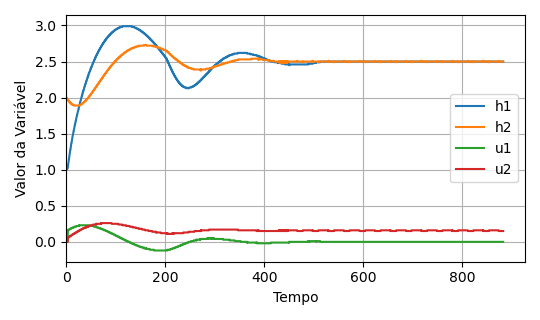
\includegraphics{PID_sem_restricoes}
	\caption{Resposta do processo para controlador PI, desconsiderando restrições de processo}
	\label{img_pid_sem_restricoes}
\end{figure}

Em seu estado estacionário, pode-se afirmar que o sistema se comporta satisfatoriamente. Como calculado no item \ref{comportamento_esperado}, com os setpoints de altura iguais, a bomba 1 tem estado estacionário nulo, e o sistema se mantém pela ação única da bomba 2, que assume um valor constante de $k \sqrt{\rho g{h_2}_{ss}} = 0,16$.

Como esperado, entretanto, o controle não é perfeito, pois não somente o sistema leva cerca de 10 minutos para estabilizar, como também tem comportamento dinâmico oscilatório, o que não corresponde com um sistema de primeira ordem. Porém, pelo controlador ter sido sintonizado considerando um sistema não linear, mas ter sido aplicado em outro não linear, o comportamento estacionário tem peso maior avaliação da eficiência do controle. Outro fator a ser considerado é acoplamento do sistema, que dificulta o controle preciso, já que cada controlador age somente sobre uma variável.

Apesar de nenhuma altura extrapolar o limite máximo de 4 metros, o sinal de controle assume, por vezes valores negativos. Se possíveis, isto sigificaria que o fluido poderia ser retirado do tanque pelas bombas, o que não ocorre neste caso. Assim, foram incluídas as seguintes restrições no processo:

\begin{enumerate}
	\item As alturas ${h_1}_{ss}$ e ${h_2}_{ss}$ devem estar compreendidas no intervalo [0, 4]m
	\item A entrada do sistema assume valores somente entre 0 e 1 $m^3/s$
\end{enumerate}

Os resultados para um sistema fisicamente mais fiel são apresentados na Figura abaixo:

\begin{figure}[H]
	\centering
	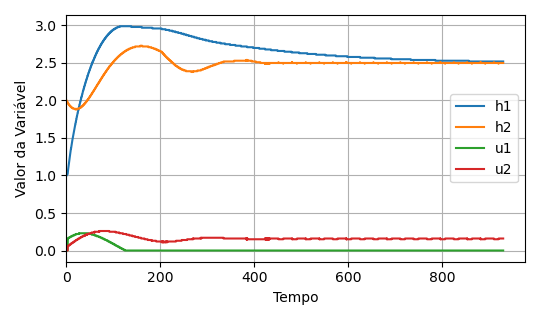
\includegraphics{PID_com_restricoes}
	\caption{Resposta do processo para controlador PI, incluindo restrições de processo}
	\label{img_pid_com_restricoes}
\end{figure}

Neste caso, para valores negativos da variável de controle, os mesmo são por sua vez substituídos por 0. Isto faz com que a altura ${h_1}_{ss}$ leve mais tempo para diminuir seu valor, pois depende somente do escoamento por gravidade e da alimentação do tanque 2. Isso se reflete no tempo de estabilização do processo em si que também é aumentado

Contudo, ainda não houve transbordamentos e os sinais de controle não atingiram valores muito altos. Assim, pode-se concluir que a estratégia do PI sintonizado em um sistema linearizado se mostrou aplicável e razoável, pois é capaz de controlar o sistema sem causar impactos negativos.


\chapter{Conclusão}

Este trabalho teve como objetivo principal apresentar e testar um sistema supervisório didático construído em Python, que permitisse aos usuários monitorar valores recebidos pela porta serial da máquina na qual fosse executado, e ainda a criarem suas próprias séries de dados. De outra perspectiva, este trabalho almejou fomentar o emprego de tecnologias open source no ambiente acadêmico, e encorajar os estudantes do ensino superior a se familiarizarem com linguagens de programação, sobretudo Pyhton, que vem ganhando adeptos no cenário atual.

Frente aos objetivos levantados, pode-se afirmar que o presente trabalho alcançou seu propósito, como exemplificado nos casos de teste. Utilizando a ferramenta desenvolvida, o estudante pode criar um sistema físico controlado por microcontrolador, e monitorar em tempo real o comportamento deste sistema. Ainda, pode salvar o gráfico da resposta no programa e compará-lo com outros comportamentos esperados, modelados também dentro do programa.

A seção de apresentação do sistema abordou algumas técnicas adotadas na programação do software, e representa um guia para construções de GUIs utilizando a bilbioteca PyQt. Apesar de haver diversos vídeos, exemplos e tutoriais na internet tratando desta biblioteca, este trabalho se destaca não só a aplicar Python no âmbito da automação, como a enriquecer a interface com outros recursos da linguagem, como a serialização de objetos e a paralelização do código em threads.

Espera-se que o produto entregue neste trabalho de conclusão de curso seja de grande valia para os estudantes, bem como para a universidade.

\section{Trabalhos futuros}

Por se tratar de um código aberto, qualquer interessado tem a possibilidade de alterar os scripts como desejar, incluindo novas funcionalidades ou modificando as existentes. Acredita-se que, por ter sido construído em uma linguagem open-source, o supervisório didático deixa muitas possibilidades de melhoria, como as citadas a seguir, ordenadas por complexidade:

\begin{enumerate}
	\item Permitir que o usuário exporte os resultados em diferentes formatos de arquivos;
	\item Adicionar um módulo no programa responsável pela escrita em um banco de dados das séries registradas, assim como feito em sistemas SCADA industriais;
	\item Criar, separadamente do supervisório, um objeto que emule um CLP;
	\item Incluir novos meios de comunicação com periféricos, como por bluetooth ou rede Wi-Fi;
	\item Acrescentar novas formas de simulação de sistemas, não somente por funções de transferência simples, mas por equações descritivas, ou até mesmo um ambiente que monte um diagrama de blocos, como implementado por ferramentas como o MATLab\textsuperscript{\tiny \textregistered} e o SciLab;
	\item Incluir ferramentas de análise de processos como perditor de Smith e estimadores e avaliadores de estado.
\end{enumerate}

\backmatter

%\bibliographystyle{abnt-alf}
% INCLUA AQUI O SEU ARQUIVO DE REFERÊNCIA
\bibliography{bibliografia.bib}

\appendix
\addcontentsline{toc}{chapter}{Anexos e Apêndices}

\chapter{Tutorial de utilização do supervisório didático} \label{Chap:Apendice1}

\section{Apresentação}

Esta seção contém um guia de utilização do supervisório didático, organizado em tópicos. Cada tópico descreve um passo-a-passo sobre como realizar as operações que o programa oferta.

\section {Primeira utilização}

O supervisório didático foi programado em linguagem Python e dividido em alguns arquivos, a fins de organização. Estes arquivos são agrupados e referenciados no script principal Supervisorio.py, sendo imprescidível que a organização dentro da pasta do programa não seja alterada. Caso seja, o script principal não conseguira encontrar os arquivos que contém as declarações de classes e será mostrado um erro no terminal.

Ao utilizar o programa, supõe-se que a máquina operante já possui Python instalado. O compilador pode ser baixado gratuitamente em \href{https://www.python.org/}{seu site oficial}. Os testes foram feitos com a versão 3.8.5 da linguagem, não sendo claros os efeitos que versões anteriores a esta causarão na operação.

Para intalação das bibliotecas utilizadas, roda-se o arquivo install\_packages.bat, presente na pasta utils. Talvez seja necessário permissão de administrador para executá-lo. Alternativamente, através do comando no código \ref{code_install_packages}, as bibliotecas listadas em requirements.txt será instaladas.

\begin{code}
	\begin{lstlisting}
	pip install -r requirements.txt
	\end{lstlisting}
	\label{code_install_packages}
\end{code}

\section{Iniciando o programa}

O script principal pode ser executado através de vários métodos, pois trata-se apenas de um script python. Para uma maneira rápida de fazê-lo, basta executar Supervisorio.bat. Ele não deve ser movido da pasta, mas pode ser criado um atalho para ele.

Quando o script é executado, a tela principal do supervisório aparecerá. Caso esteja presente um arquivo de salvamento automático autosave.dat no diretório raiz do programa, ele tentará restaurar as séries da sessão anterior. Caso apareçam erros no trecho que carrega estes dados, o usuário pode tentar deletar este arquivo.

\section{Importando séries estáticas no programa}

Existem diversos métodos de entrada de dados no supervisório. Primeiro, alguns parâmetros são configurados, de acordo com cada método, descritos nas subseções posteriores, e depois clica-se no botão "Puxar Dados".

\subsection{Função de Transferência}

A simulação de funções de tranferência no programa requer o numerador e denominador de cada função, multiplicadas entre sim, bem como o estado inicial da saída do sistema e o ganho do degrau aplicado. Para este método, o sistema reponde somente a uma entrada degrau. A entrada de dados por função de transferência se dá pelo objeto ilustrado na Figura \ref{img_transfer_func_config}.

\begin{figure}[!htb]
	\centering
	\caption{Objeto \emph{TransferFunctionConfig} (à esquerda)}
	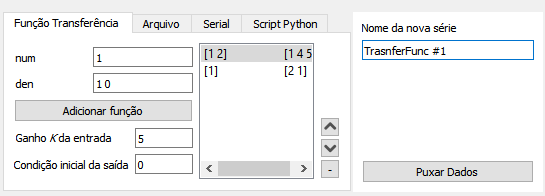
\includegraphics{transfer_func_config}
	\label{img_transfer_func_config}
\end{figure}

Com o campo num e den preenchidos com uma sequência de números separados por espaço, clica-se no botão "Adicionar Função" para incluí-la na lista à direita. Cada número é atribuído em ordem de posição a uma potência de s, sendo o número mais à direita atribuído a $s^0$. Como exemplo, um numerador "1 3" e denominador "2 0 1" representam a função de transferência $\frac{s + 3}{2s^2 + 1}$.

\textbf{OBS:} o numerador não pode ter grau maior que o denominador, por restrições da biblioteca empregada neste módulo.

A ordem das funções não impacta a resposta final, mas por questão de organização, foram incluídos botões à direita da tabela que mudam a posição de cada função na lista. O botão "-" remove a função selecionada, se houver, da mesma.

Terminada a entrada de funções de transferência, configuram-se o estado inicial e o ganho do degrau. Após isto, clica-se no botão "Puxar Dados"

\subsection{Entrada por arquivo}

O programa aceita 4 formatos de arquivos para inserção de séries, que são .csv, .tsv, .xls e .xslx. Todos estes formatos armazenam dados em tabela, logo compartilham seus parâmetros de importação:

\begin{itemize}
	\item \textbf{Cabeçalho:} Caso a opção "Considerar cabeçalho" seja marcada, o programa transformará a primeira linha de dados lida como a lista de nomes de cada série.
	\item \textbf{Eixo de tempo:} Com a opção "1ª coluna como eixo de tempo", o programa considerará a coluna mais a esquerda como eixo de tempo, compartilhado pelas outras séries contidas no arquivo. Caso a opção marcada seja "Gerar eixo de tempo autom.", o programa criaré este eixo pela quantidade de linhas lidas, começando em 1, e em incrementos unitários a cada leitura.
\end{itemize}

Na parte superior do objeto \emph{FileConfig}, são listados cada um dos formatos compatíveis com o programa. O formato selecionado configura o filtro de extensão do explorador de arquivos que aparece quando o botão "..." é clicado. Ao selecionar um arquivo por este explorador, o programa preencherá automaticamente os campos "Diretório" e "Arquivo".

\subsection{Serial}

A importação por porta serial é configurada pelos seguintes parâmetros:

\begin{itemize}
	\item \textbf{\emph{baud rate}}: velocidade de recebimento e transmissão dos dados na porta;
	\item \textbf{Porta}: nome da porta;
	\item \textbf{\emph{timeout}}: tempo máximo de resposta do dispositivo conectado, quando a comunicação for iniciada.
	\item \textbf{N\# colunas} quantas séries de dados recebidas devem ser esperadas pelo programa, incluindo a série de tempo. Após cada leitura da porta serial, se a quantidade de valores lidos diferir deste número, a leitura será desconsiderada.
\end{itemize}

Abaixo de algumas configurações existe uma lista com os valores mais populares de parâmetros. Ao clicar nos itens da lista, a caixa de texto será atualizada. O botão "Testar" abre e fecha uma conexão na porta informada, a fim de verificar se não houve problemas.

Para este caso, ao iniciar a importação, a janela de monitoramento irá aparecer, como descrito na seção \ref{monitoramento_tempo_real}.

\subsection{Script Python}

Esta alternativa busca oferecer aos usuários maneiras próprias de criação de dados. Na caixa de texto pode ser digitado um script python que retorne, nesta ordem, uma lista de séries, um eixo de tempo e uma lista de nomes. O programa criará um objeto \emph{SeriesObject} a partir do retorno deste script. Ainda é possível clicar duplamente na caixa de texto, momento no qual uma caixa maior aparece, garantindo maior visibilidade. Nela há também alguns exemplo de códigos, que podem ser modificados livremente pelo usuário.

A puxar dados de um script python, o programa escreve o texto em um arquivo denominado script.py, em seu diretório raiz, cuidando de toda a sixtaxe adicional. Em seguida, envia um comando ao sistema operacional para executar o script final, que armazena o resultado em um objeto serializado. Por fim, este objeto é decodificado e, caso não hajam erros, uma nova série é criada.

\section{Monitoramento em tempo real}\label{monitoramento_tempo_real}

Ao clicar em "Puxar Dados" por porta serial, o programa tenta estabelecer uma conexão com os parâmetros informados, na porta definida. O nome da porta pode variar com o sistema operacional.

Após a conexão ser estabelecida, o programa limpará qualquer informação escrita no buffer da porta e, em intervalos de 2 segundos nela escreverá "go", até que alguma informação de retorno seja recebida. Isso se repetirá até 100 vezes. Este procedimento por ser alterado na função \emph{setup\_connection()} do objeto SCADADialog, presente no script realtime\_objects.py na pasta objects.

Após esta rotina de sincronização, a função personalizada setup\_control() é chamada. Caso o usuário deseje enviar algum valor para o controlador (setpoints, parâmetros do sistema, entre  outros), deve fazê-lo por aqui. O programa abre também a janela de monitoramento \emph{SCADADialog}, com um gráfico que plota cada série de dados recebida em tempo real.

Finalmente, iniciam-se as rotinas de leitura da porta e atualização do gráfico, respectivamente a cada 0,2 e 1 segundo. Como mencionado, a rotina de leitura lê toda uma linha de dados da porta, divide-a pelas tabulações contidas, e atribui cada trecho a uma série de dados interna, sendo a primeira sempre o eixo de tempo. Este formato deve ser seguido pelo emissor, ou controlador, acoplado, pois caso não coincida com a quantidade de séries esperada passado como parâmetro, toda a linha será ignorada.

Contida na rotina de leitura está a função loop\_control(). Idealmente, ela tem como objetivo mandar valores para o controlador em tempo de execução.

Durante o monitoramento, o usuário pode interromper a execução ao clicar em "Parar" ou "Cancelar". O segundo fecha a janela de monitoramento e descarta a série armazenada até então. O primeiro somente interrompe u fluxo de dados, e possibilita que o usuário salve as séries lidas, clicando em "Criar Série".

\section{Salvando e editando séries de dados}

Qualquer que tenha sido o método de importação, o usuário terá uma visualização dos dados importados sempre antes de efetivamente salvá-los no programa. Isto é ilustrado na Figura \ref{img_edit_series_dialog}. 

Nesta caixa diálogo, o usuário pode editar o título do conjunto e cabeçalho de cada série sendo importada. Para editar o cabeçalho, clica-se no nome da série contido na tabela à esquerda e altera-se a caixa de texto imediatamente acima dela. Cada alteração deve ser confirmada com Enter.

Após realizadas as edições, o usuário pode clicar em "Criar Série", e ela aparecerá na lista de séries à direita da aplicação pricipal.

Para editar uma série já criada, clica-se no respectivo botão "Editar", na lista de série, e esta mesma janela aparecerá. Para este caso, o botão "Criar Série" será substituído por "Salvar Alterações".

\section{Plotando séries}

A plotagem de séries na área principal se dá clicando em "Plotar", momento no qual o gráfico no canto inferior esquerdo da aplicação desenhará a série, sem perder outras já plotadas. A legenda também será atualizada.

\section{Editando e exportando gráficos}

Abaixo da área de plotagem, existe uma barra com algumas opções de configurações, como:

\begin{itemize}
	\item 
\includegraphics[height=1em]{zoom_icon} Permite aplicar zoom no gráfico
	\item 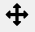
\includegraphics[height=1em]{move_icon} Permite mover o gráfico
	\item 
\includegraphics[height=1em]{home_icon} Retorna o gráfico à escala original
	\item 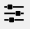
\includegraphics[height=1em]{limits_icon} Configura o espaçamento do gráfico e sua moldura
	\item 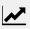
\includegraphics[height=1em]{axes_icon} Configura os eixos do gráfico, editando seu rótulo, limites e escala
	\item 
\includegraphics[height=1em]{save_icon} Salva o gráfico em formato de imagem
\end{itemize}

\section{Deletando séries}

Ao clicar em "Deletar", a série é apagada. Esta operação é irreversível.
\chapter{Tutorial de utilização do supervisório didático} \label{Chap:Apendice2}

\section{Apresentação}

Esta seção contém um guia de utilização do supervisório didático, organizado em tópicos. Cada tópico descreve um passo-a-passo sobre como realizar as operações que o programa oferta.

\section {Primeira utilização}

O supervisório didático foi programado em linguagem Python e dividido em alguns arquivos, a fins de organização. Estes arquivos são agrupados e referenciados no script principal Supervisorio.py, sendo imprescidível que a organização dentro da pasta do programa não seja alterada. Caso seja, o script principal não conseguira encontrar os arquivos que contém as declarações de classes e será mostrado um erro no terminal.

Ao utilizar o programa, supõe-se que a máquina operante já possui Python instalado. O compilador pode ser baixado gratuitamente em \href{https://www.python.org/}{seu site oficial}. Os testes foram feitos com a versão 3.8.5 da linguagem, não sendo claros os efeitos que versões anteriores a esta causarão na operação.

Para intalação das bibliotecas utilizadas, roda-se o arquivo install\_packages.bat, presente na pasta utils. Talvez seja necessário permissão de administrador para executá-lo. Alternativamente, através do comando \ref{code_install_packages}, as bibliotecas listadas em requirements.txt será instaladas.

\begin{code}
\begin{lstlisting}
pip install -r requirements.txt
\end{lstlisting}
\label{code_install_packages}
\end{code}

\section{Iniciando o programa}

O script principal pode ser executado através de vários métodos, pois trata-se apenas de um script python. Para uma maneira rápida de fazê-lo, basta executar Supervisorio.bat. Ele não deve ser movido da pasta, mas pode ser criado um atalho para ele.

Quando o script é executado, a tela principal do supervisório aparecerá. Caso esteja presente um arquivo de salvamento automático autosave.dat no diretório raiz do programa, ele tentará restaurar as séries da sessão anterior. Caso apareçam erros no trecho que carrega estes dados, o usuário pode tentar deletar este arquivo.

\section{Importando séries estáticas no programa}

Existem diversos métodos de entrada de dados no supervisório. Primeiro, alguns parâmetros são configurados, de acordo com cada método, descritos nas subseções posteriores, e depois clica-se no botão "Puxar Dados".

\subsection{Função de Transferência}

A simulação de funções de tranferência no programa requer o numerador e denominador de cada função, multiplicadas entre sim, bem como o estado inicial da saída do sistema e o ganho do degrau aplicado. Para este método, o sistema reponde somente a uma entrada degrau. A entrada de dados por função de transferência se dá pelo objeto ilustrado na Figura \ref{img_transfer_func_config}.

\begin{figure}[!htb]
	\centering
	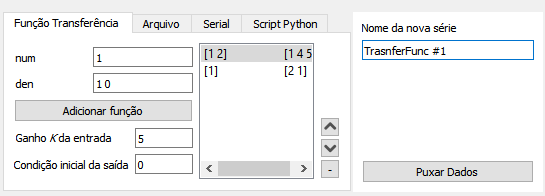
\includegraphics{transfer_func_config}
	\caption{Objeto \emph{TransferFunctionConfig} (à esquerda)}
	\label{img_transfer_func_config}
\end{figure}

Com o campo num e den preenchidos com uma sequência de números separados por espaço, clica-se no botão "Adicionar Função" para incluí-la na lista à direita. Cada número é atribuído em ordem de posição a uma potência de s, sendo o número mais à direita atribuído a $s^0$. Como exemplo, um numerador "1 3" e denominador "2 0 1" representam a função de transferência $\frac{s + 3}{2s^2 + 1}$.

\textbf{OBS:} o numerador não pode ter grau maior que o denominador, por restrições da biblioteca empregada neste módulo.

A ordem das funções não impacta a resposta final, mas por questão de organização, foram incluídos botões à direita da tabela que mudam a posição de cada função na lista. O botão "-" remove a função selecionada, se houver, da mesma.

Terminada a entrada de funções de transferência, configuram-se o estado inicial e o ganho do degrau. Após isto, clica-se no botão "Puxar Dados"

\subsection{Entrada por arquivo}

O programa aceita 4 formatos de arquivos para inserção de séries, que são .csv, .tsv, .xls e .xslx. Todos estes formatos armazenam dados em tabela, logo compartilham seus parâmetros de importação:

\begin{itemize}
	\item \textbf{Cabeçalho:} Caso a opção "Considerar cabeçalho" seja marcada, o programa transformará a primeira linha de dados lida como a lista de nomes de cada série.
	\item \textbf{Eixo de tempo:} Com a opção "1ª coluna como eixo de tempo", o programa considerará a coluna mais a esquerda como eixo de tempo, compartilhado pelas outras séries contidas no arquivo. Caso a opção marcada seja "Gerar eixo de tempo autom.", o programa criaré este eixo pela quantidade de linhas lidas, começando em 1, e em incrementos unitários a cada leitura.
\end{itemize}

Na parte superior do objeto \emph{FileConfig}, são listados cada um dos formatos compatíveis com o programa. O formato selecionado configura o filtro de extensão do explorador de arquivos que aparece quando o botão "..." é clicado. Ao selecionar um arquivo por este explorador, o programa preencherá automaticamente os campos "Diretório" e "Arquivo".

\subsection{Serial}

A importação por porta serial é configurada pelos seguintes parâmetros:

\begin{itemize}
	\item \textbf{\emph{baud rate}}: velocidade de recebimento e transmissão dos dados na porta;
	\item \textbf{Porta}: nome da porta;
	\item \textbf{\emph{timeout}}: tempo máximo de resposta do dispositivo conectado, quando a comunicação for iniciada.
	\item \textbf{N\# colunas} quantas séries de dados recebidas devem ser esperadas pelo programa, incluindo a série de tempo. Após cada leitura da porta serial, se a quantidade de valores lidos diferir deste número, a leitura será desconsiderada.
\end{itemize}

Abaixo de algumas configurações existe uma lista com os valores mais populares de parâmetros. Ao clicar nos itens da lista, a caixa de texto será atualizada. O botão "Testar" abre e fecha uma conexão na porta informada, a fim de verificar se não houve problemas.

Para este caso, ao iniciar a importação, a janela de monitoramento irá aparecer, como descrito na seção \ref{monitoramento_tempo_real}.

\subsection{Script Python}

Esta alternativa busca oferecer aos usuários maneiras próprias de criação de dados. Na caixa de texto pode ser digitado um script python que retorne, nesta ordem, uma lista de séries, um eixo de tempo e uma lista de nomes. O programa criará um objeto \emph{SeriesObject} a partir do retorno deste script. Ainda é possível clicar duplamente na caixa de texto, momento no qual uma caixa maior aparece, garantindo maior visibilidade. Nela há também alguns exemplo de códigos, que podem ser modificados livremente pelo usuário.

A puxar dados de um script python, o programa escreve o texto em um arquivo denominado script.py, em seu diretório raiz, cuidando de toda a sixtaxe adicional. Em seguida, envia um comando ao sistema operacional para executar o script final, que armazena o resultado em um objeto serializado. Por fim, este objeto é decodificado e, caso não hajam erros, uma nova série é criada.

\section{Monitoramento em tempo real}\label{monitoramento_tempo_real}

Ao clicar em "Puxar Dados" por porta serial, o programa tenta estabelecer uma conexão com os parâmetros informados, na porta definida. O nome da porta pode variar com o sistema operacional.

Após a conexão ser estabelecida, o programa limpará qualquer informação escrita no buffer da porta e, em intervalos de 2 segundos nela escreverá "go", até que alguma informação de retorno seja recebida. Isso se repetirá até 100 vezes. Este procedimento por ser alterado na função \emph{setup\_connection()} do objeto SCADADialog, presente no script realtime\_objects.py na pasta objects.

Após esta rotina de sincronização, a função personalizada setup\_control() é chamada. Caso o usuário deseje enviar algum valor para o controlador (setpoints, parâmetros do sistema, entre  outros), deve fazê-lo por aqui. O programa abre também a janela de monitoramento \emph{SCADADialog}, com um gráfico que plota cada série de dados recebida em tempo real.

Finalmente, iniciam-se as rotinas de leitura da porta e atualização do gráfico, respectivamente a cada 0,2 e 1 segundo. Como mencionado, a rotina de leitura lê toda uma linha de dados da porta, divide-a pelas tabulações contidas, e atribui cada trecho a uma série de dados interna, sendo a primeira sempre o eixo de tempo. Este formato deve ser seguido pelo emissor, ou controlador, acoplado, pois caso não coincida com a quantidade de séries esperada passado como parâmetro, toda a linha será ignorada.

Contida na rotina de leitura está a função loop\_control(). Idealmente, ela tem como objetivo mandar valores para o controlador em tempo de execução.

Durante o monitoramento, o usuário pode interromper a execução ao clicar em "Parar" ou "Cancelar". O segundo fecha a janela de monitoramento e descarta a série armazenada até então. O primeiro somente interrompe u fluxo de dados, e possibilita que o usuário salve as séries lidas, clicando em "Criar Série".

\section{Salvando e editando séries de dados}

Qualquer que tenha sido o método de importação, o usuário terá uma visualização dos dados importados sempre antes de efetivamente salvá-los no programa. Isto é ilustrado na Figura \ref{img_edit_series_dialog}. 

Nesta caixa diálogo, o usuário pode editar o título do conjunto e cabeçalho de cada série sendo importada. Para editar o cabeçalho, clica-se no nome da série contido na tabela à esquerda e altera-se a caixa de texto imediatamente acima dela. Cada alteração deve ser confirmada com Enter.

Após realizadas as edições, o usuário pode clicar em "Criar Série", e ela aparecerá na lista de séries à direita da aplicação pricipal.

Para editar uma série já criada, clica-se no respectivo botão "Editar", na lista de série, e esta mesma janela aparecerá. Para este caso, o botão "Criar Série" será substituído por "Salvar Alterações".

\section{Plotando séries}

A plotagem de séries na área principal se dá clicando em "Plotar", momento no qual o gráfico no canto inferior esquerdo da aplicação desenhará a série, sem perder outras já plotadas. A legenda também será atualizada.

\section{Editando e exportando gráficos}

Abaixo da área de plotagem, existe uma barra com algumas opções de configurações, como:

\begin{itemize}
	\item 
\includegraphics[height=1em]{zoom_icon} Permite aplicar zoom no gráfico
	\item 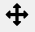
\includegraphics[height=1em]{move_icon} Permite mover o gráfico
	\item 
\includegraphics[height=1em]{home_icon} Retorna o gráfico à escala original
	\item 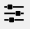
\includegraphics[height=1em]{limits_icon} Configura o espaçamento do gráfico e sua moldura
	\item 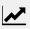
\includegraphics[height=1em]{axes_icon} Configura os eixos do gráfico, editando seu rótulo, limites e escala
	\item 
\includegraphics[height=1em]{save_icon} Salva o gráfico em formato de imagem
\end{itemize}

\section{Deletando séries}

Ao clicar em "Deletar", a série é apagada. Esta operação é irreversível.

%\includepdf{CAPA_DISSERTACAO_PEI_DANIEL_DINIZ_SANTANA_FUNDO.pdf}

\end{document}
